\documentclass[12pt,a4paper]{report}
\RequirePackage[english,spanish,brazil,portuguese]{babel}
\RequirePackage[T1]{fontenc}
\RequirePackage{graphicx}
\graphicspath{{./logotipos/}{./figuras/}}
\PassOptionsToPackage{table}{xcolor}
\RequirePackage{pdfpages}
\RequirePackage{xspace}
\RequirePackage{setspace}
\RequirePackage{geometry}
\geometry{a4paper,top=30mm,bottom=20mm,left=30mm,right=20mm}
\RequirePackage[utf8]{inputenc}
\usepackage{indentfirst}
\usepackage{multirow}
\usepackage{float}
\usepackage{longtable} 

\begin{document}
\appendix

\chapter{}

Algoritmo Genético de Regime Permanente com Contador de Ocorrências 1ª Versão

\begin{figure}[H]
\centering

\includegraphics[scale=1]{AGRPCO1/1}

\end{figure}

\begin{figure}[H]
\centering

\includegraphics[scale=1]{AGRPCO1/2}

\end{figure}

\begin{figure}[H]
\centering

\includegraphics[scale=1]{AGRPCO1/3}

\end{figure}
\begin{figure}[H]
\centering

\includegraphics[scale=1]{AGRPCO1/4}

\end{figure}
\begin{figure}[H]
\centering

\includegraphics[scale=1]{AGRPCO1/5}

\end{figure}
\begin{figure}[H]
\centering

\includegraphics[scale=1]{AGRPCO1/6}

\end{figure}
\begin{figure}[H]
\centering

\includegraphics[scale=1]{AGRPCO1/7}

\end{figure}
\begin{figure}[H]
\centering

\includegraphics[scale=1]{AGRPCO1/8}

\end{figure}
\begin{figure}[H]
\centering

\includegraphics[scale=1]{AGRPCO1/9}

\end{figure}
\begin{figure}[H]
\centering

\includegraphics[scale=1]{AGRPCO1/10}

\end{figure}

Algoritmo Genético de Regime Permanente com Contador de Ocorrências 2ª Versão

\begin{figure}[H]
\centering

\includegraphics[scale=1]{AGRPCO2/1}

\end{figure}

\begin{figure}[H]
\centering

\includegraphics[scale=1]{AGRPCO2/2}

\end{figure}

\begin{figure}[H]
\centering

\includegraphics[scale=1]{AGRPCO2/3}

\end{figure}

\begin{figure}[H]
\centering

\includegraphics[scale=1]{AGRPCO2/4}

\end{figure}

\begin{figure}[H]
\centering

\includegraphics[scale=1]{AGRPCO2/5}

\end{figure}

\begin{figure}[H]
\centering

\includegraphics[scale=1]{AGRPCO2/6}

\end{figure}

\begin{figure}[H]
\centering

\includegraphics[scale=1]{AGRPCO2/7}

\end{figure}

\begin{figure}[H]
\centering

\includegraphics[scale=1]{AGRPCO2/8}

\end{figure}

\begin{figure}[H]
\centering

\includegraphics[scale=1]{AGRPCO2/9}

\end{figure}

\begin{figure}[H]
\centering

\includegraphics[scale=1]{AGRPCO2/10}

\end{figure}


\end{document}